\section{产品原型}

借助墨刀进行设计,最终的原型分享链接为:\url{https://modao.cc/app/uz2y2AfIrk37uvQr6iMQ7R}

原型页面如下:\\


\iffalse

\begin{figure}[h!]
    \centering
    
\includegraphics[width=\linewidth]{imgs/prototype/home.png}
    \caption{登录流程}
    \label{fig:loginflow}
\end{figure}

\fi

首页,可以通过两个按钮进入 login/register 页面,也可以点击三角形查看平台介绍

\begin{figure}[h!]
    \centering
    
\includegraphics[width=\linewidth]{imgs/prototype/home.png}
    \caption{首页}
    \label{fig:proto_home}
\end{figure}

\newpage

平台介绍页面,包括联系方式以及设计团队等等

\begin{figure}[h!]
    \centering
    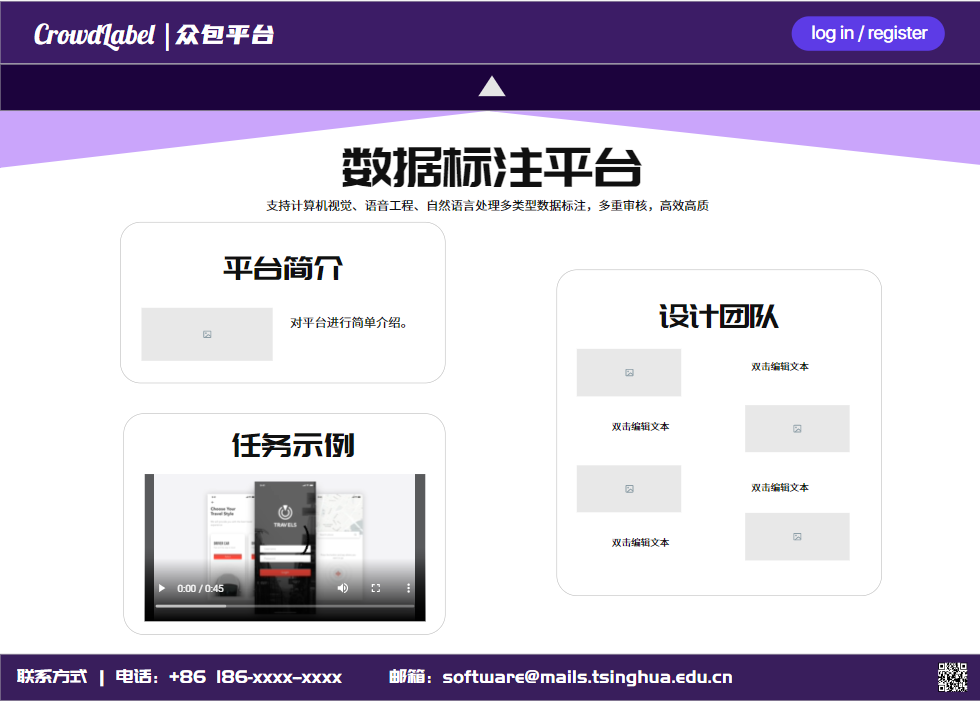
\includegraphics[width=\linewidth]{imgs/prototype/description.png}
    \caption{平台介绍页面}
    \label{fig:proto_description}
\end{figure}

\newpage

通过按钮进入到用户类型选择界面,随后可以点击屏幕中按钮

\begin{figure}[h!]
    \centering
    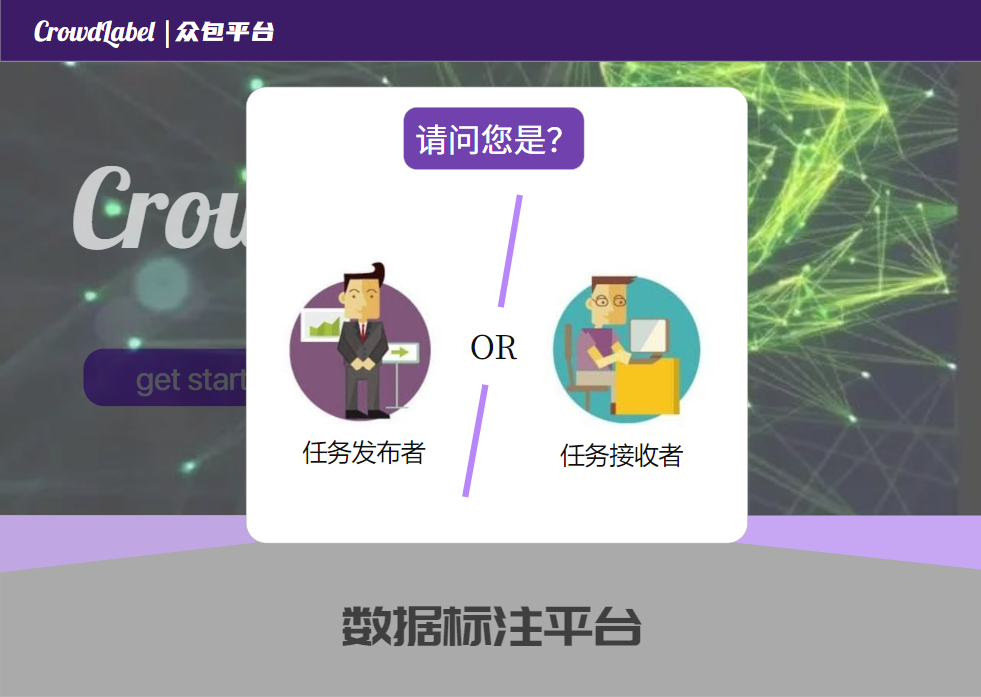
\includegraphics[width=\linewidth]{imgs/prototype/profile.png}
    \caption{用户类型选择界面}
    \label{fig:proto_profile}
\end{figure}

\newpage

Login 和 Sign up 界面,通过点击上方的按钮进行相应的操作

\begin{figure}[h!]
    \centering
    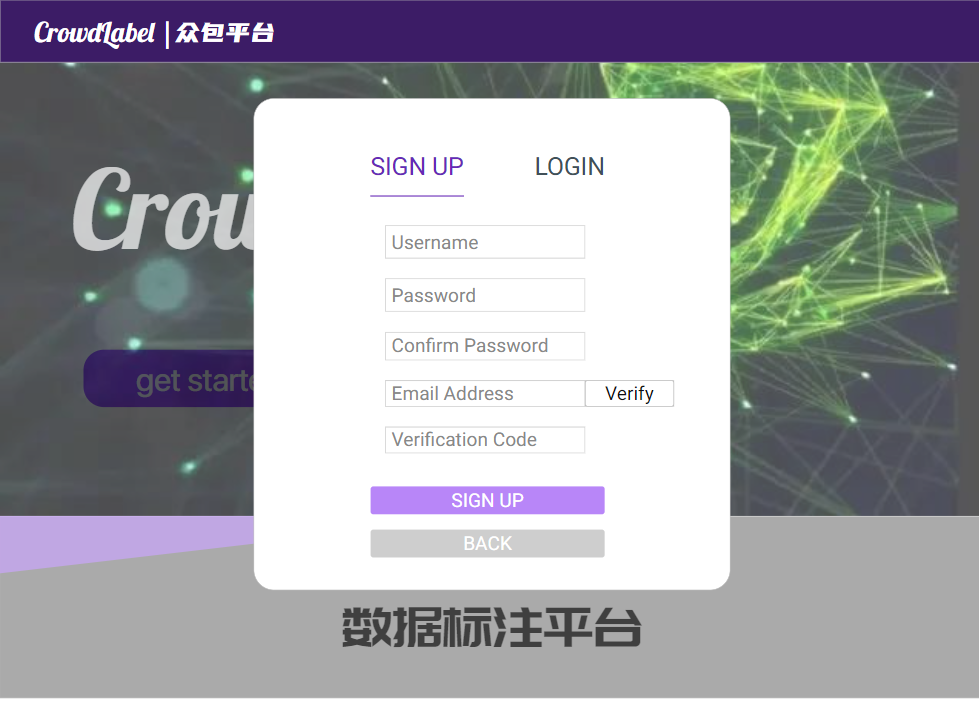
\includegraphics[width=\linewidth]{imgs/prototype/register.png}
    \caption{用户类型选择界面}
    \label{fig:proto_register}
\end{figure}


\newpage

任务接收方的任务大厅页面

\begin{figure}[h!]
    \centering
    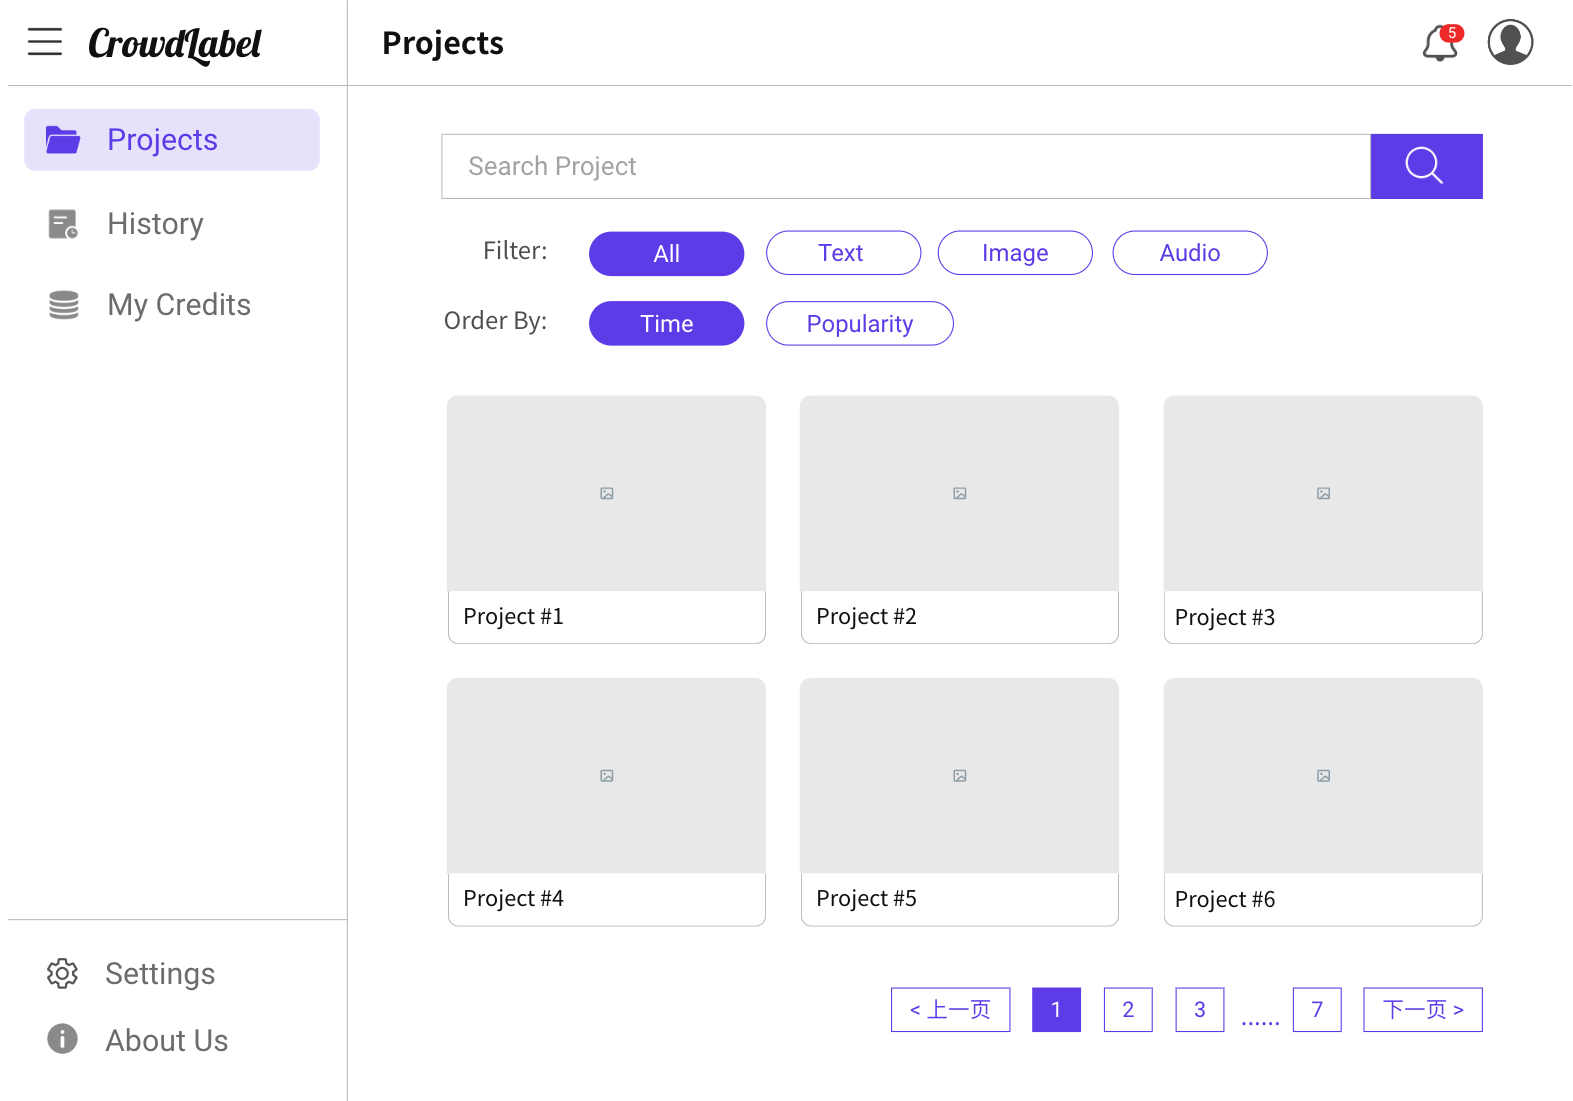
\includegraphics[width=\linewidth]{imgs/prototype/list.png}
    \caption{任务大厅}
    \label{fig:proto_list}
\end{figure}

\newpage

点击特定任务,跳转至任务详情页面

\begin{figure}[h!]
    \centering
    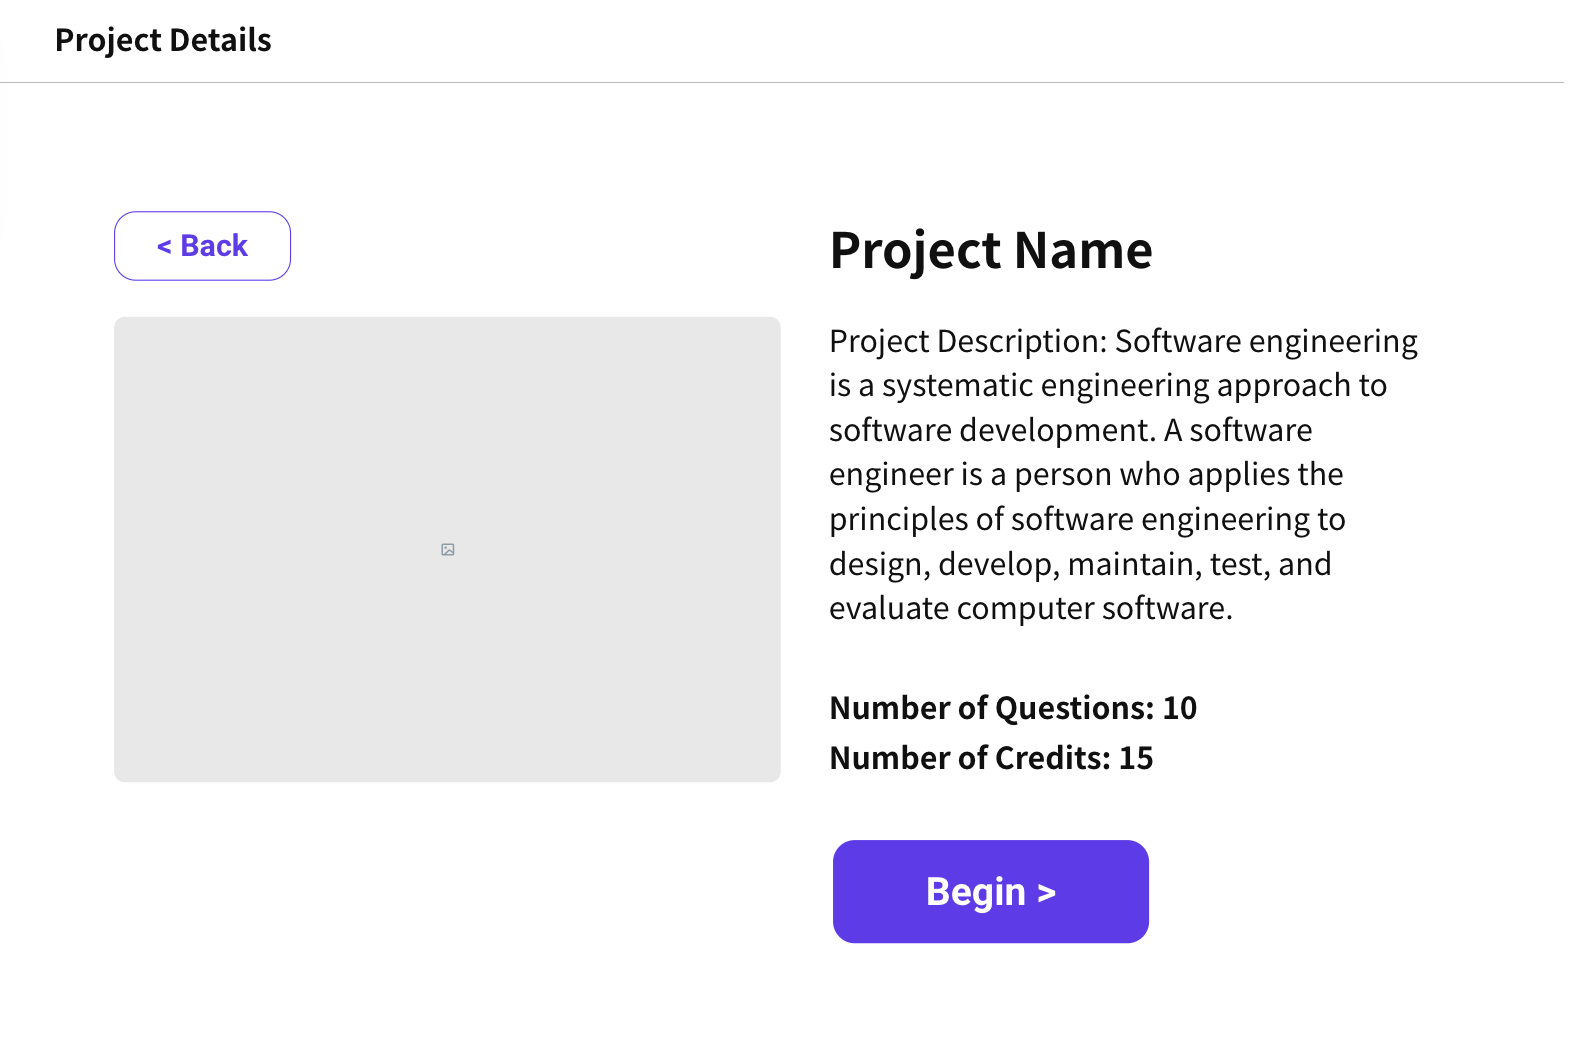
\includegraphics[width=\linewidth]{imgs/prototype/task_description.png}
    \caption{任务详情}
    \label{fig:proto_task_description}
\end{figure}

\newpage

任务发送方的主界面

\begin{figure}[h!]
    \centering
    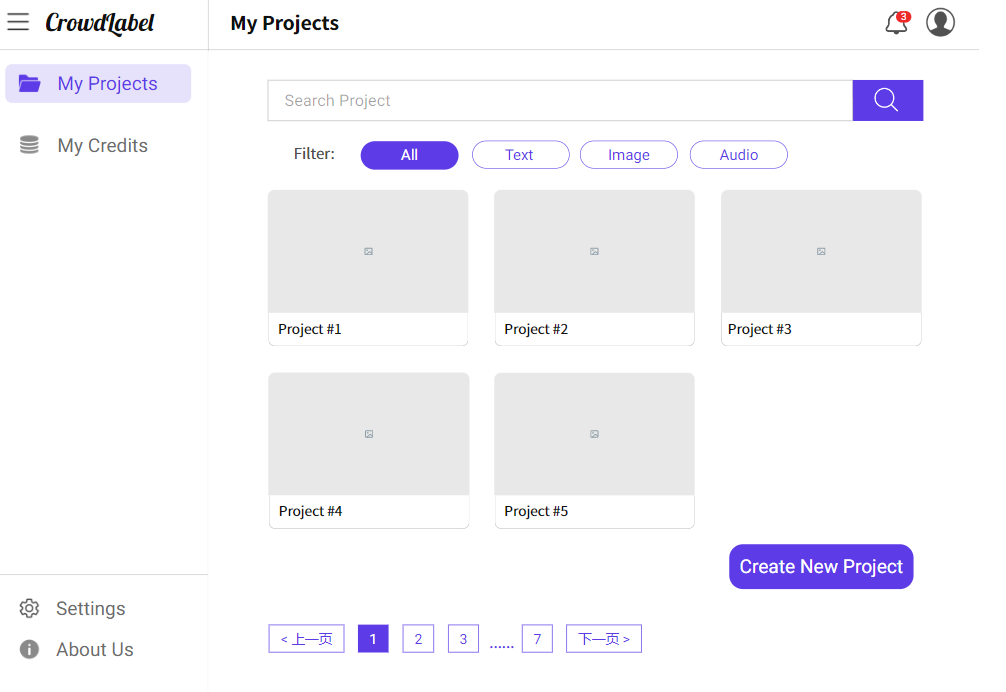
\includegraphics[width=\linewidth]{imgs/prototype/myprojects.png}
    \caption{任务发送方的主界面}
    \label{fig:proto_myprojects}
\end{figure}

\newpage

任务打标过程页面示例:文本标注

\begin{figure}[h!]
    \centering
    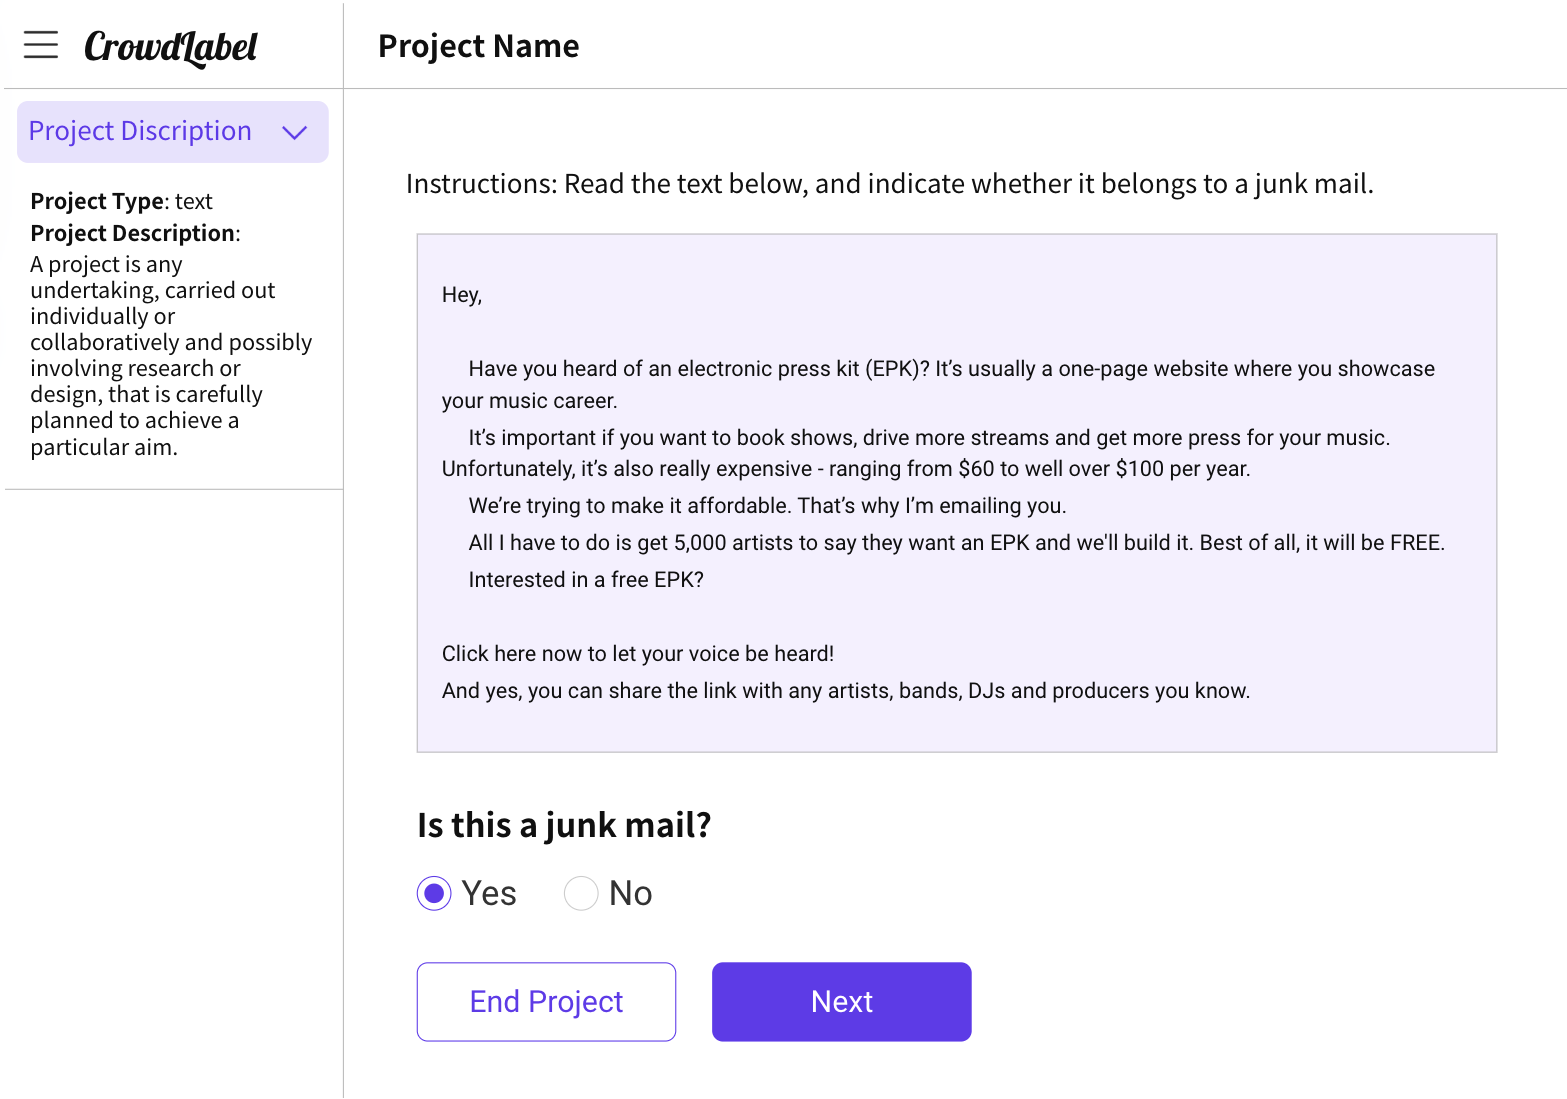
\includegraphics[width=\linewidth]{imgs/prototype/text.png}
    \caption{文本标注}
\end{figure}

\newpage

任务打标过程页面示例:图像标注

\begin{figure}[h!]
    \centering
    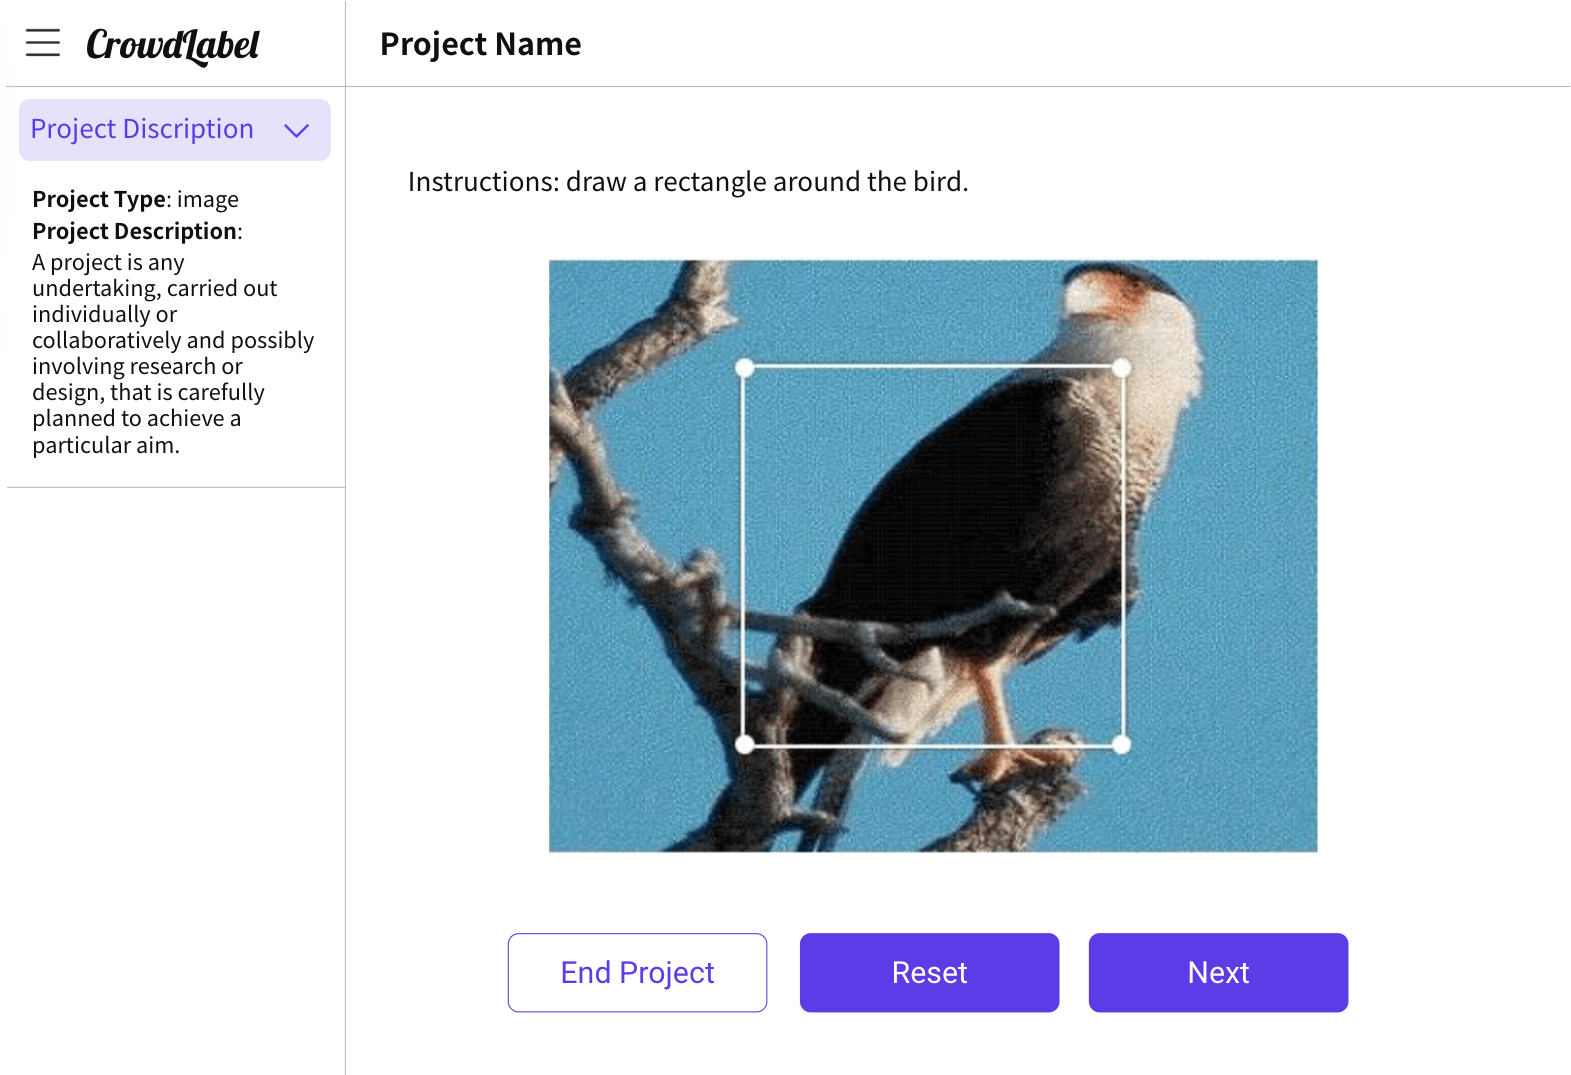
\includegraphics[width=\linewidth]{imgs/prototype/img.png}
    \caption{图像标注}
\end{figure}

\newpage

任务打标过程页面示例:音频标注

\begin{figure}[h!]
    \centering
    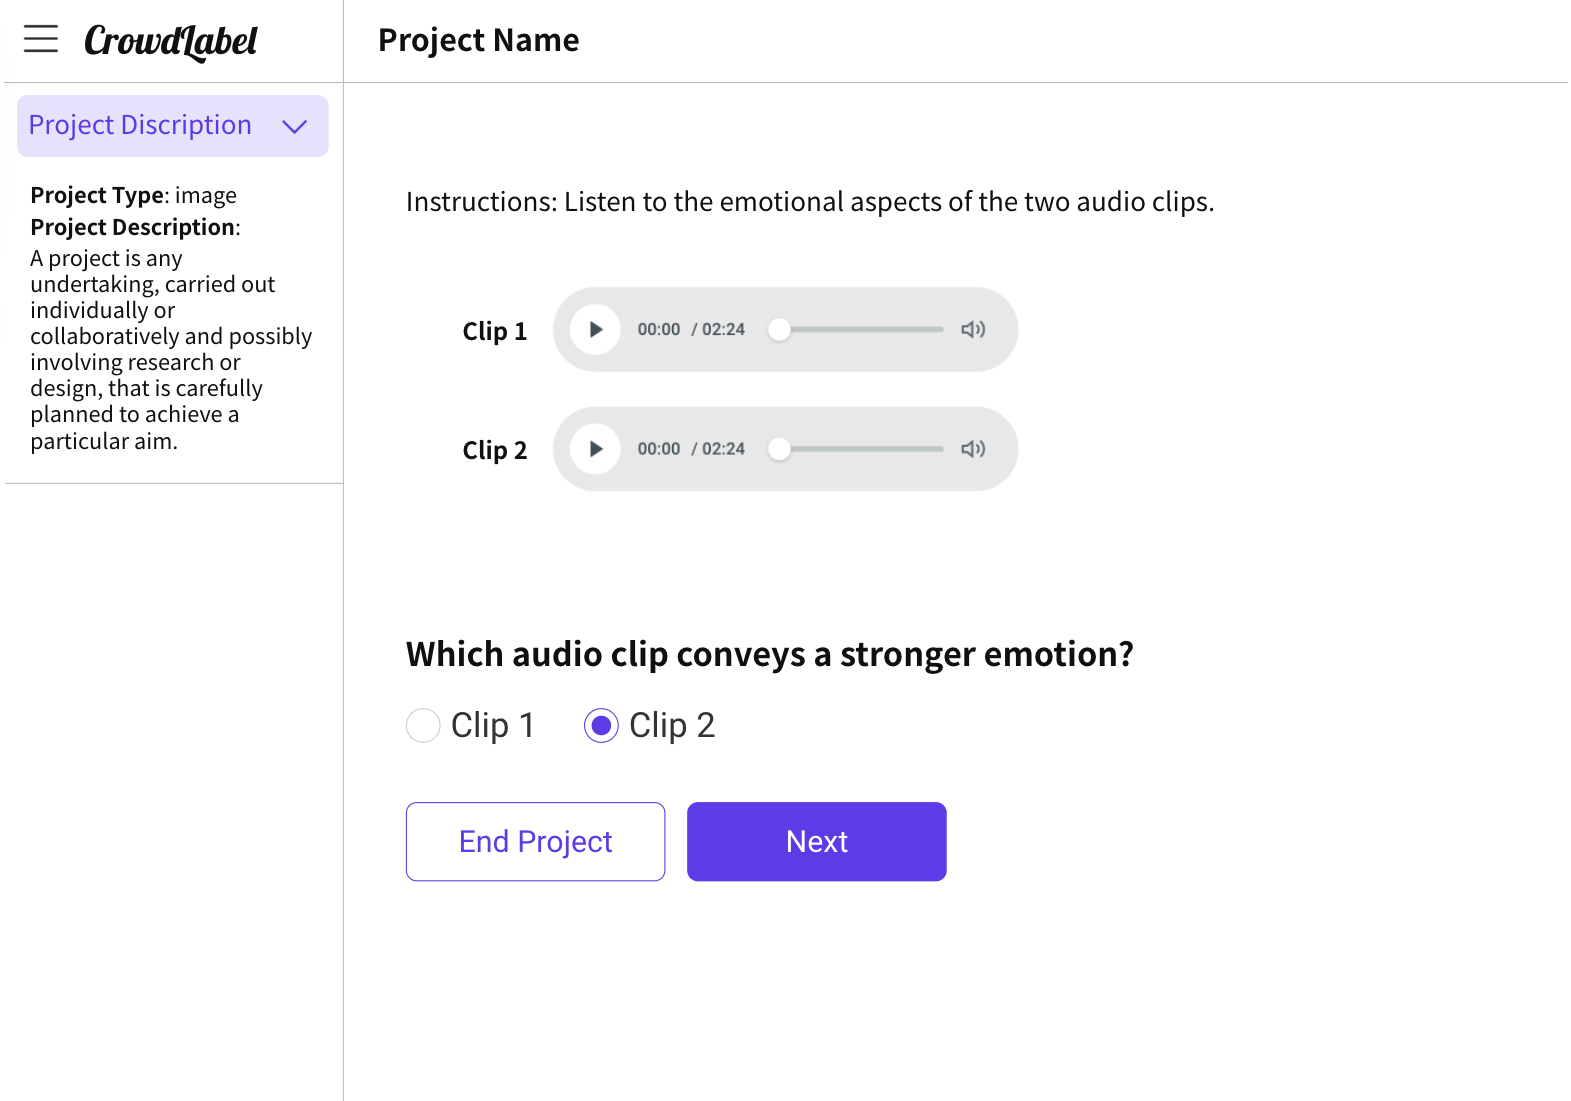
\includegraphics[width=\linewidth]{imgs/prototype/audio.png}
    \caption{音频标注}
\end{figure}

\newpage

任务完成界面,提示用户等待打标审核结果通知

\begin{figure}[h!]
    \centering
    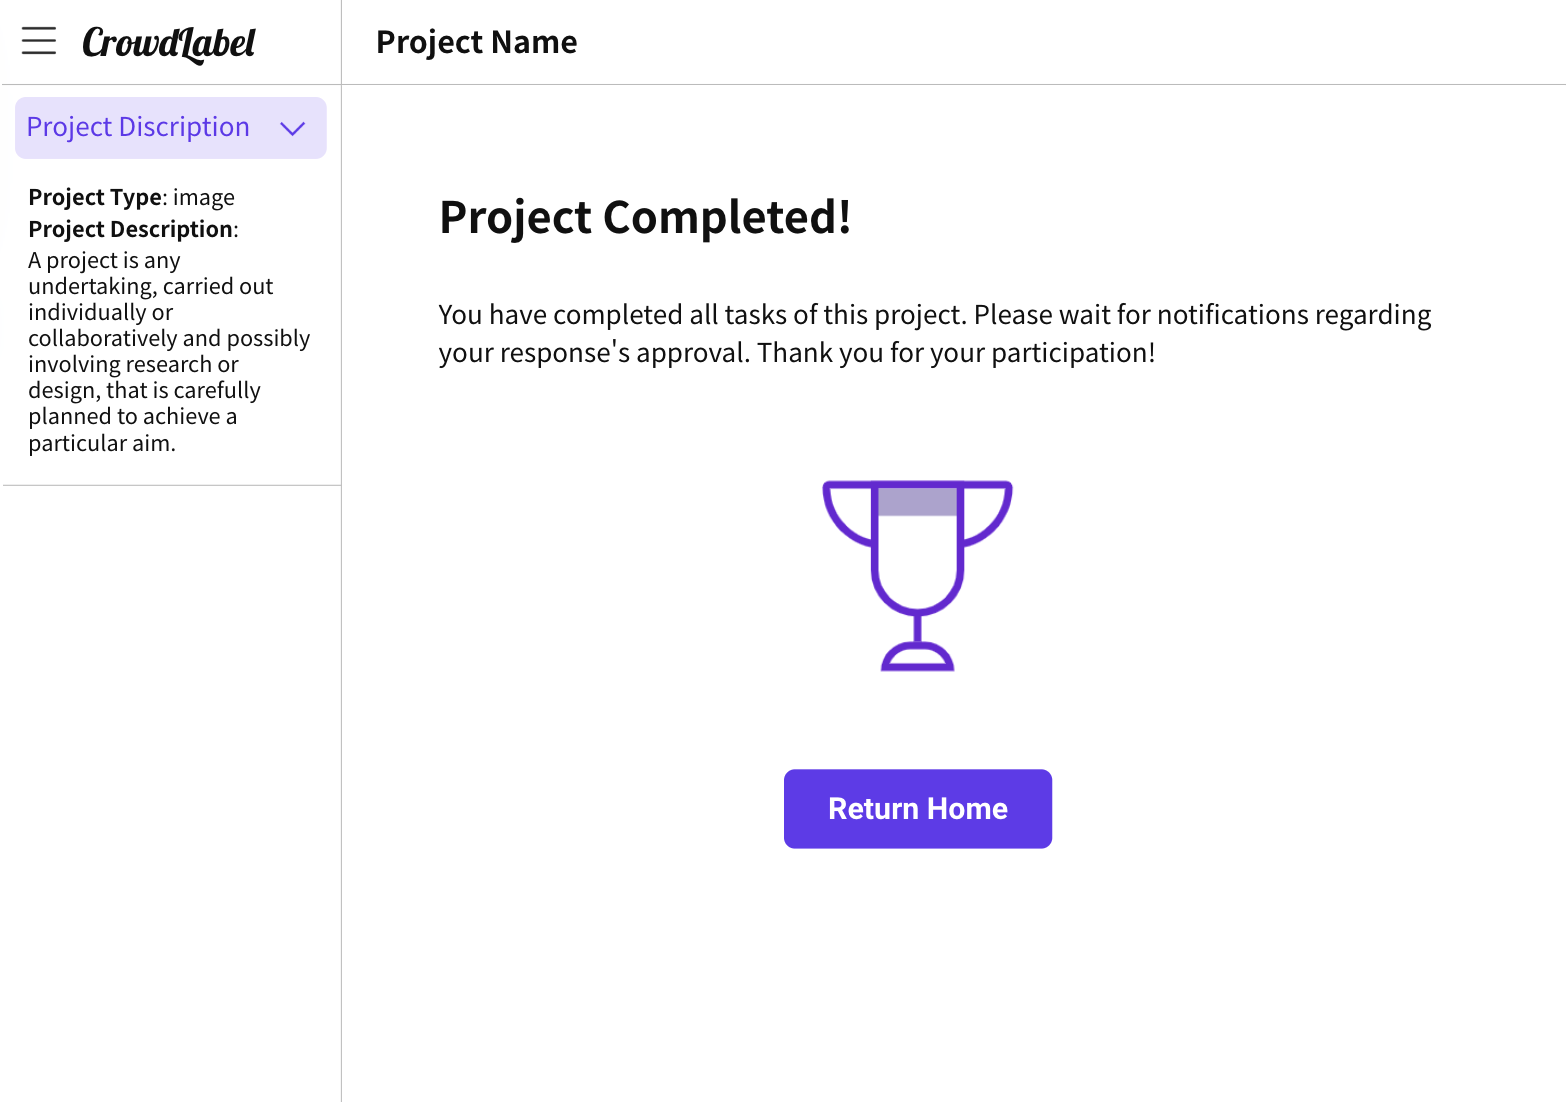
\includegraphics[width=\linewidth]{imgs/prototype/completed.png}
    \caption{任务完成}
\end{figure}

\newpage

在首页查看新消息通知

\begin{figure}[h!]
    \centering
    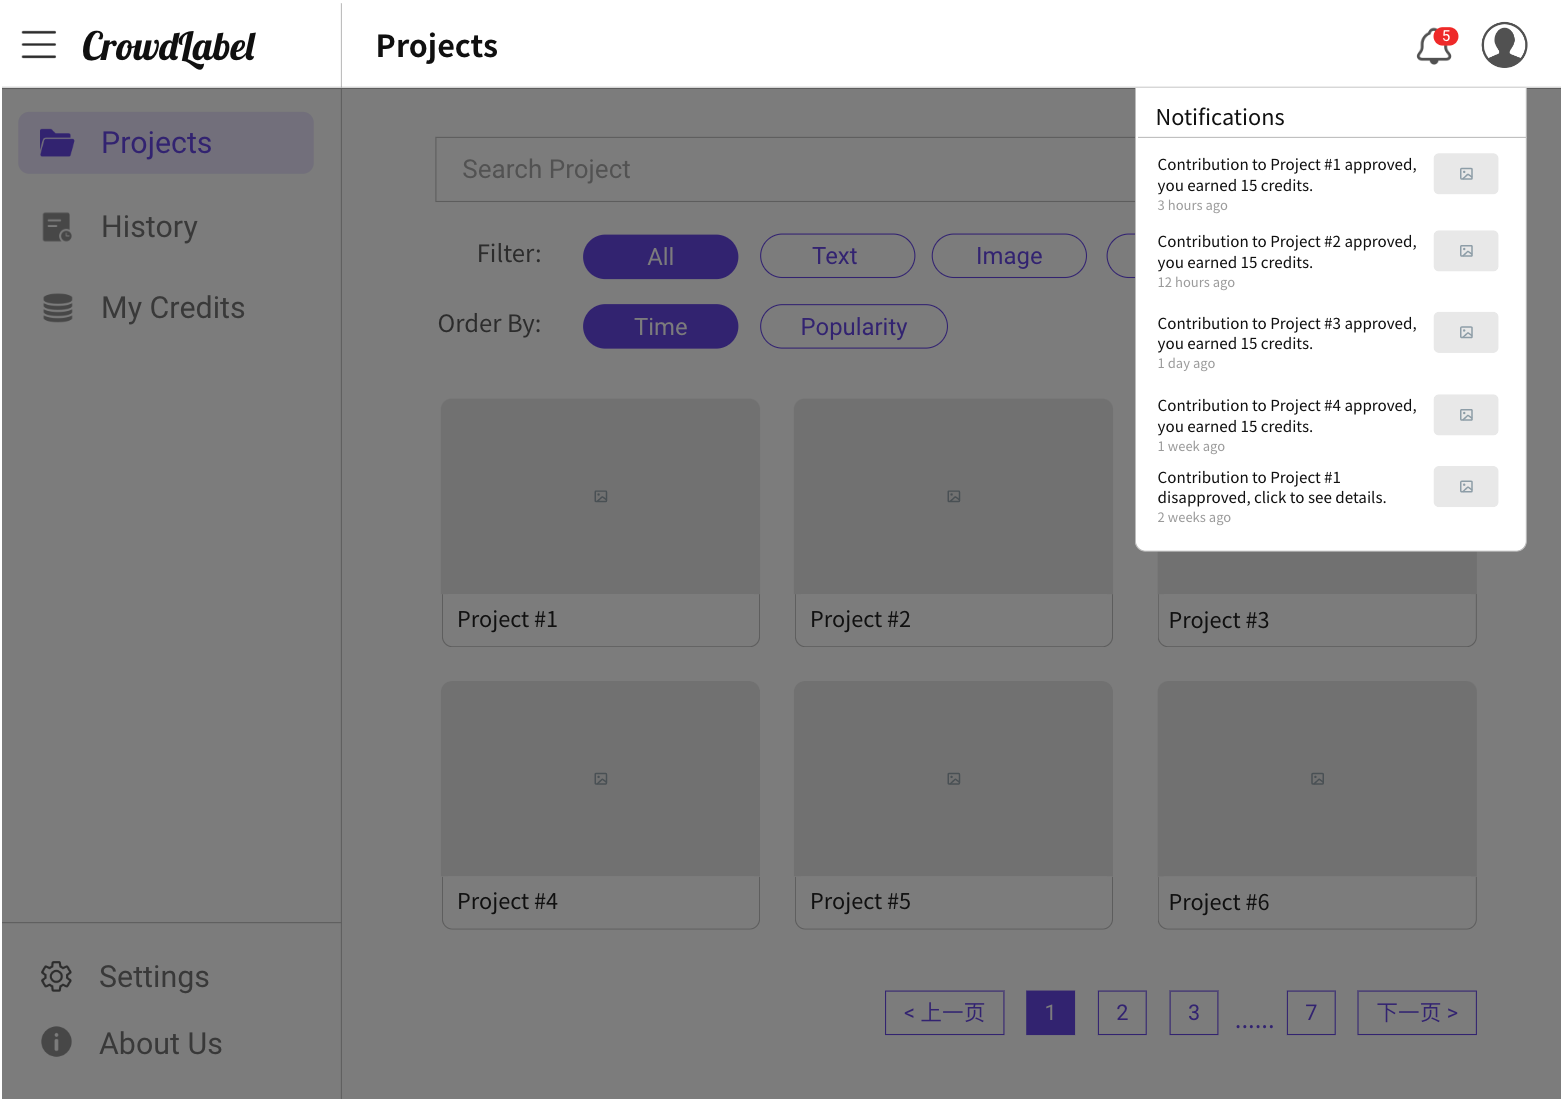
\includegraphics[width=\linewidth]{imgs/prototype/notifs.png}
    \caption{消息通知}
\end{figure}

\newpage

查看并修改个人信息

\begin{figure}[h!]
    \centering
    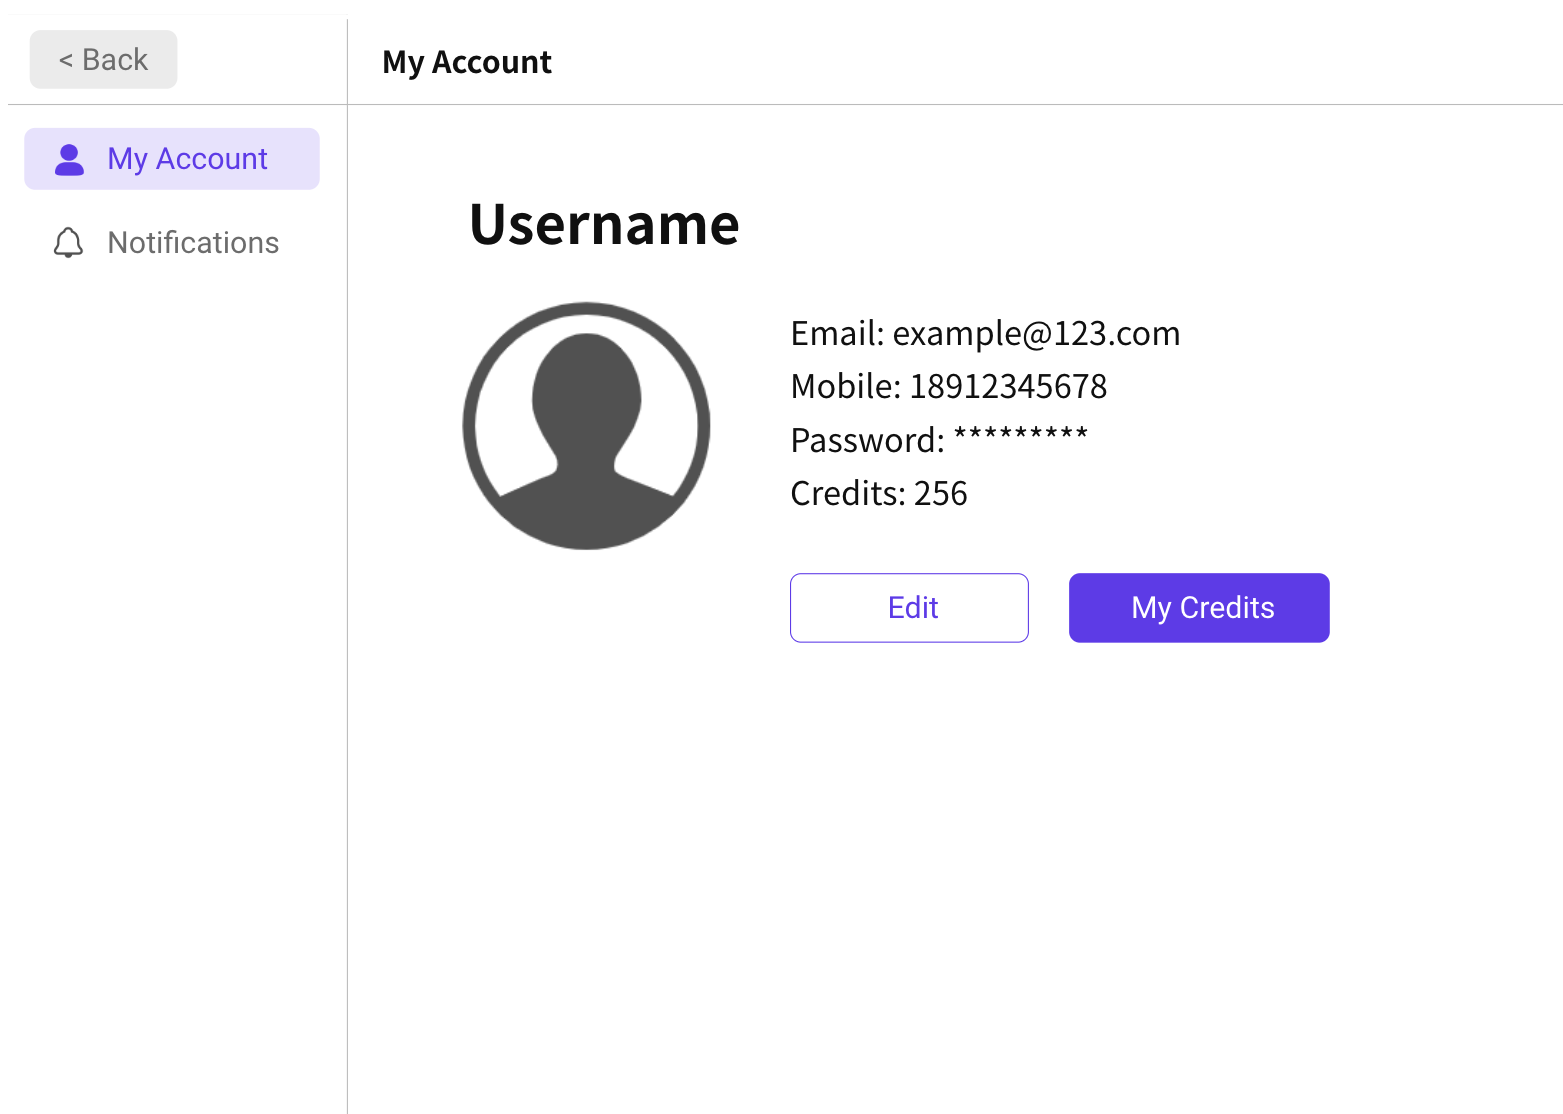
\includegraphics[width=\linewidth]{imgs/prototype/myaccount.png}
    \caption{个人信息}
\end{figure}

\newpage

查看积分并提现

\begin{figure}[h!]
    \centering
    
\includegraphics[width=\linewidth]{imgs/prototype/credits.png}
    \caption{任务接收者的积分}
\end{figure}

\newpage

新建项目页面,可以选择项目类型,并且之后跳转到积分奖励选择界面

\begin{figure}[h!]
    \centering
    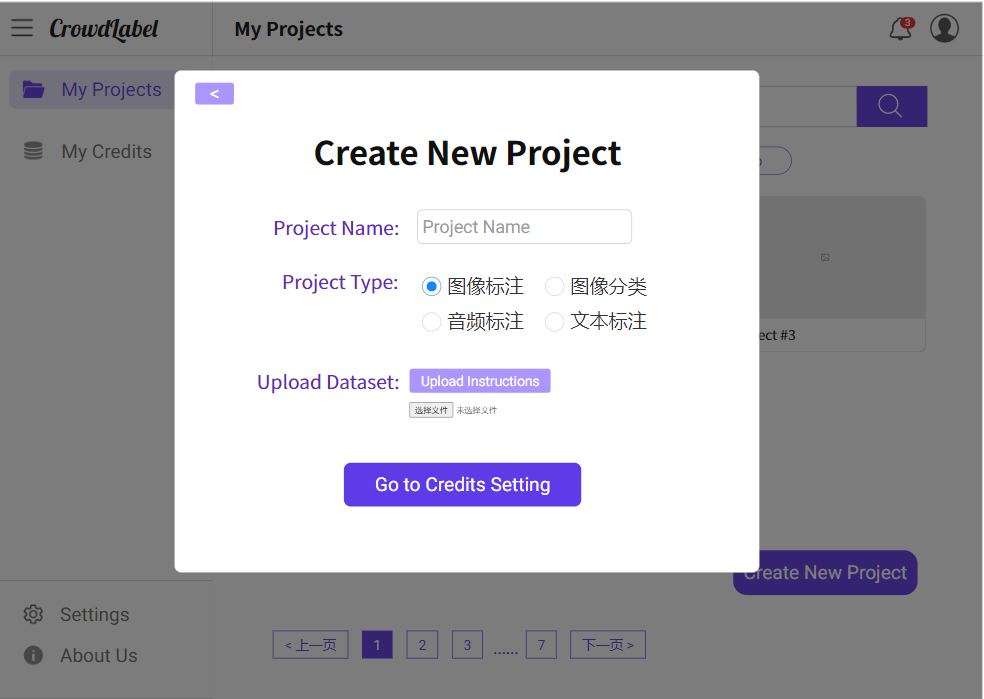
\includegraphics[width=\linewidth]{imgs/prototype/newproject.png}
    \caption{新建项目}
\end{figure}

\newpage

任务发放者的积分界面,通过充值(top up)的方式获得积分

\begin{figure}[h!]
    \centering
    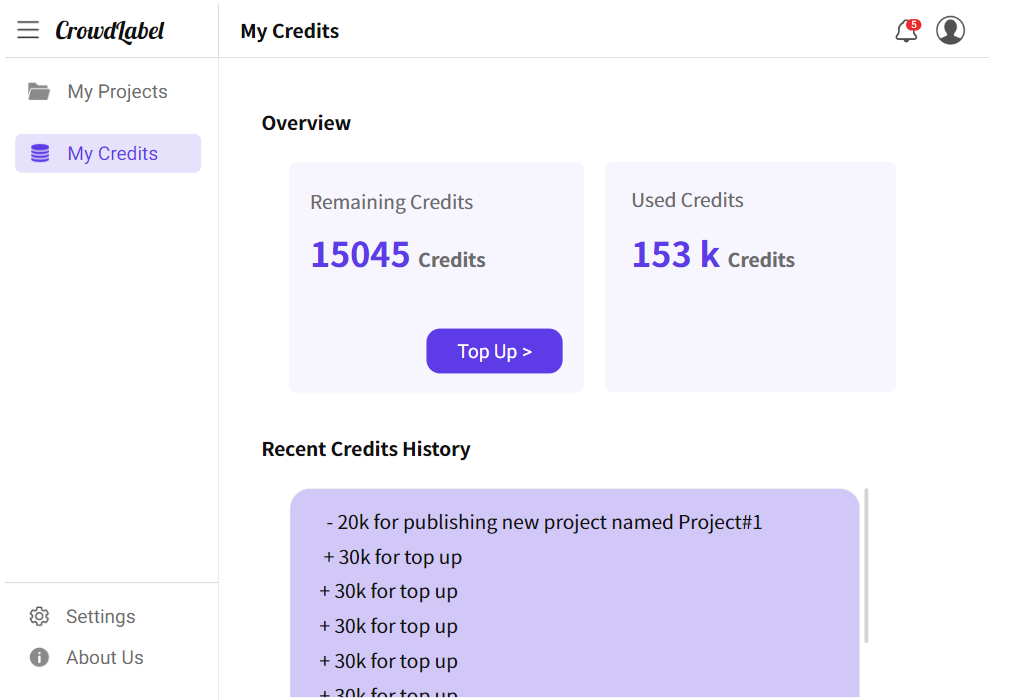
\includegraphics[width=\linewidth]{imgs/prototype/sendercredits.png}
    \caption{任务发放者的积分}
\end{figure}